% =============================================================================
%  Paper 011 — Continuous Performance & Drift Monitoring for Deployed Clinical Agents
%  QUOKKAGUARD program. House style derived from papers/_template (QFIRE paper).
%  Build:  make   (tectonic preferred; falls back to pdflatex+bibtex)
% =============================================================================
\documentclass[11pt]{article}
\usepackage[utf8]{inputenc}
\usepackage[margin=1in]{geometry}
\usepackage{booktabs}
\usepackage{graphicx}
\usepackage{float}
\usepackage{afterpage}
\usepackage[section]{placeins}
\renewcommand{\topfraction}{0.9}
\renewcommand{\bottomfraction}{0.8}
\renewcommand{\textfraction}{0.08}
\renewcommand{\floatpagefraction}{0.75}
\setcounter{topnumber}{3}
\setcounter{bottomnumber}{2}
\setcounter{totalnumber}{5}
\usepackage{amsmath}
\usepackage{amssymb}
\usepackage{hyperref}
\usepackage{xcolor}
\usepackage{listings}
\definecolor{kwblue}{rgb}{0.10,0.20,0.65}
\definecolor{typepurple}{rgb}{0.50,0.15,0.55}
\definecolor{strred}{rgb}{0.62,0.12,0.12}
\definecolor{cmtgreen}{rgb}{0.20,0.45,0.20}
\lstdefinestyle{housespecyaml}{
  basicstyle=\ttfamily\footnotesize,
  backgroundcolor=\color{black!3},
  frame=single,
  framesep=5pt,
  rulecolor=\color{black!45},
  columns=fullflexible,
  breaklines=true,
  keepspaces=true,
  showstringspaces=false,
  alsoletter=_,
  commentstyle=\color{cmtgreen}\itshape,
  stringstyle=\color{strred},
  morecomment=[l]{\#},
  morestring=[b]",
  morestring=[b]',
  keywordstyle=\color{kwblue}\bfseries,
  keywords={detector,signal,window,envelope,ladder,threshold,warmup},
  keywordstyle=[2]\color{typepurple}\bfseries,
  keywords=[2]{cusum,adwin,conformal,distdistance,notify,throttle,halt},
}
\lstdefinestyle{housespecyamlbare}{style=housespecyaml, frame=none,
  backgroundcolor=\color{white}, xleftmargin=0pt, framexleftmargin=0pt,
  aboveskip=1pt, belowskip=0pt}
\usepackage[most]{tcolorbox}
\tcbuselibrary{listings,skins}
\usepackage{tikz}
\usetikzlibrary{positioning,shapes.geometric,arrows.meta,calc,fit,backgrounds,shadows}
\definecolor{cardindigo}{HTML}{4F46E5}
\definecolor{slate}{HTML}{475569}
\definecolor{amber}{HTML}{D97706}
\definecolor{cardblue}{HTML}{1D4ED8}
\definecolor{cardpurple}{HTML}{6D28D9}
\definecolor{cardteal}{HTML}{0F766E}
\tcbset{
  cardcol/.store in=\cardcol, cardcol=cardblue,
  policycard/.style={
    enhanced, breakable=false, arc=3pt, boxrule=0.7pt, top=3pt, bottom=3pt,
    left=7pt, right=7pt, boxsep=1pt, coltitle=white,
    colframe=\cardcol!60!black, colback=white, colbacktitle=\cardcol,
    fonttitle=\bfseries\small, drop fuzzy shadow=black!25,
  },
}
\usepackage{url}
\usepackage{multirow}
\usepackage{array}
\usepackage{ragged2e}
\newcolumntype{L}[1]{>{\RaggedRight\arraybackslash}p{#1}}
\usepackage[htt]{hyphenat}
\hypersetup{colorlinks=true, linkcolor=blue, citecolor=blue, urlcolor=blue}
\usepackage{caption}
\DeclareCaptionLabelFormat{boldunder}{\underline{\textbf{#1~#2}}}
\captionsetup{font=small, labelformat=boldunder, labelsep=colon,
  textfont=normalcolor, skip=6pt}
\let\oldincludegraphics\includegraphics
\renewcommand{\includegraphics}[2][]{%
  \setlength{\fboxsep}{0pt}\setlength{\fboxrule}{0.5pt}%
  \fbox{\oldincludegraphics[#1]{#2}}}
\newcommand{\todofig}[2]{%
  \begin{tcolorbox}[colback=black!4, colframe=black!35, arc=3pt, boxrule=0.5pt,
    halign=center, valign=center, height=#1, width=\linewidth]
    {\ttfamily\small [FIGURE PLACEHOLDER]\\[4pt] #2}
  \end{tcolorbox}}
\providecommand{\NumPrompts}{0}
\providecommand{\NumAttacks}{0}
\providecommand{\NumBenign}{0}
\IfFileExists{numbers.tex}{% Headline numbers for paper 011 (continuous performance & drift monitoring).
% Every reported number in main.tex resolves to a macro here, so the prose stays
% traceable to the run. Source: HAARF-Drift (seed 42), results/011-drift-monitoring/.
% Core macros are \providecommand'd in main.tex -> override with \renewcommand;
% all new result macros use \newcommand.
\renewcommand{\NumPrompts}{168}   % total streams in HAARF-Drift
\renewcommand{\NumAttacks}{102}   % onset/creep/anomaly streams (54 + 24 + 24)
\renewcommand{\NumBenign}{66}     % clean streams (18 + 24 + 24)

% --- Corpus composition ---
\newcommand{\Seed}{42}
\newcommand{\StreamLen}{1000}     % cases per stream
\newcommand{\DriftOnset}{54}      % drift streams with an injected onset
\newcommand{\DriftClean}{18}
\newcommand{\AutoCreep}{24}
\newcommand{\AutoClean}{24}
\newcommand{\BehAnom}{24}
\newcommand{\BehClean}{24}

% --- E1 drift detection (detection rate over 54 onset streams) ---
\newcommand{\CusumDet}{54/54}
\newcommand{\AdwinDet}{36/54}
\newcommand{\ConfDet}{54/54}
\newcommand{\DistDet}{54/54}
% per-magnitude mean detection latency (cases): small / med / large
\newcommand{\CusumLatSmall}{8.1}
\newcommand{\CusumLatMed}{2.2}
\newcommand{\CusumLatLarge}{1.0}
\newcommand{\ConfLatSmall}{33.2}
\newcommand{\ConfLatMed}{19.3}
\newcommand{\ConfLatLarge}{19.0}
\newcommand{\DistLatSmall}{15.0}
\newcommand{\DistLatMed}{5.9}
\newcommand{\DistLatLarge}{5.7}
\newcommand{\AdwinLatMed}{115.2}
\newcommand{\AdwinLatLarge}{28.7}
% ROC AUC
\newcommand{\CusumAUC}{1.00}
\newcommand{\AdwinAUC}{0.83}
\newcommand{\ConfAUC}{1.00}
\newcommand{\DistAUC}{1.00}

% --- E2 delayed/partial labels (outcome-CUSUM) ---
\newcommand{\EtwoFullRate}{0.72}   % full labels, no delay
\newcommand{\EtwoFullLat}{60}      % cases
\newcommand{\EtwoSparseRate}{0.56} % frac 0.2
\newcommand{\EtwoSparseLat}{214}
\newcommand{\EtwoDelayLat}{210}    % delay 150, full frac
\newcommand{\EtwoMaxLat}{364}      % delay 150 + frac 0.2
\newcommand{\EtwoMaxFAR}{0.056}

% --- E3 autonomy creep ---
\newcommand{\AutoRecall}{1.00}
\newcommand{\AutoFAR}{0.00}
\newcommand{\AutoLat}{0.2}          % cases past onset
\newcommand{\AutoEnvLo}{0.4}
\newcommand{\AutoEnvHi}{0.7}

% --- E4 unsupervised behavioral anomaly ---
\newcommand{\BehRecall}{1.00}
\newcommand{\BehFPRsens}{0.42}      % threshold 0.2 (too sensitive)
\newcommand{\BehThreshOp}{0.5}      % operating threshold
\newcommand{\BehFPRop}{0.00}        % at threshold >= 0.35
\newcommand{\BehLatOp}{14.8}        % cases at operating threshold

% --- E5 overhead (us/event; representative run, deterministic detection) ---
\newcommand{\OvCusum}{0.007}
\newcommand{\OvConf}{0.034}
\newcommand{\OvAdwin}{0.19}
\newcommand{\OvDist}{0.22}
\newcommand{\AdwinBuckets}{53}
\newcommand{\OvEvents}{72000}

% --- Implementation ---
\newcommand{\MonitorTests}{16}      % monitor module unit tests
\newcommand{\NumDetectors}{4}
}{}
\newcommand{\monthyeartoday}{%
  \ifcase\month\or January\or February\or March\or April\or May\or June\or
  July\or August\or September\or October\or November\or December\fi
  \space\number\year}

\begin{document}

% ============================================================================
% Title page
% ============================================================================
\thispagestyle{empty}
\noindent
\begin{minipage}[c]{0.55\textwidth}
  \raggedright\oldincludegraphics[height=1.05cm]{figs/quome.png}
\end{minipage}\hfill
\begin{minipage}[c]{0.4\textwidth}
  \raggedleft\itshape\large \monthyeartoday
\end{minipage}

\vspace{1.1em}
\begin{center}
  {\LARGE\bfseries Watching the Deployment, Not the Call:\\[2pt]
   Continuous Performance and Drift Monitoring for Deployed Clinical Agents\par}

  \vspace{0.9em}
  {\large
   Jim Schwoebel\textsuperscript{1,\,*}\quad
   QUOKKAGUARD Contributors\textsuperscript{1}\par}

  \vspace{0.7em}
  {\small
   \textsuperscript{1}\,Quome\par}
  \vspace{0.35em}
\end{center}

\vspace{0.5em}
\begin{tcolorbox}[breakable, enhanced jigsaw, colback=black!4, colframe=black!4,
  arc=5pt, boxrule=0pt, left=16pt, right=16pt, top=10pt, bottom=10pt]
\setlength{\parskip}{0pt}
{\centering\large\bfseries Abstract\par}
\smallskip
\fontsize{9.5}{11.3}\selectfont
A clinical agent that is safe at release does not stay safe. Practice patterns shift,
populations change, an upstream model is swapped beneath it, or an attacker reshapes
its behavior gradually to stay under per-call detectors. The prior layers of this
program decide \emph{each call} --- they firewall prompts~\cite{schwoebel2026qfire}, attest the
harness~\cite{pristineweights2026}, make the action log non-repudiable~\cite{tamperaudit2026},
authorize tools in context~\cite{policy2026}, control data egress~\cite{egress2026}, and
bind agent identity~\cite{multiagent2026} --- but \emph{nothing watches the deployment
over time}. We build \textbf{\texttt{qfire monitor}}, an off-hot-path layer that consumes
the signed decision stream and runs sequential, memory-bounded detectors for three
deployment failure modes: performance drift, autonomy creep, and behavioral anomaly. We
release \textbf{HAARF-Drift}, a deterministic, fully synthetic benchmark of \NumPrompts{}
temporal agent-decision streams (\StreamLen{} cases each) with labeled, injected
drift/creep/anomaly episodes of known onset and magnitude. \textbf{Headline:} across four
drift detectors, \emph{no single detector dominates} --- CUSUM detects an injected
degradation within \CusumLatLarge{}--\CusumLatSmall{} cases (large$\to$small magnitude,
ROC AUC \CusumAUC{}), while ADWIN is robust but conservative on small drift
(AUC \AdwinAUC{}). Autonomy-creep monitoring reaches \AutoRecall{} recall at \AutoFAR{}
false-alarm rate; an \emph{unsupervised} behavioral monitor reaches \BehRecall{} recall at
\BehFPRop{} false-positive rate \emph{with no labels} --- the regime where outcome-based
monitoring degrades (detection falls to \EtwoSparseRate{} and latency rises to
\EtwoMaxLat{} cases under delayed/partial labels). All detectors run at sub-microsecond
to \OvDist~\textmu s per event with bounded memory. The central result: deployment-time
safety needs \emph{several complementary signals}, including a label-free one, because
the failure that hides from outcomes is exactly the one an adversary aims for. All code,
data, and result artifacts are released; all data are synthetic.

\medskip
\noindent\textbf{Keywords:}~drift detection; post-market surveillance; autonomy
monitoring; concept drift; conformal martingales; clinical AI safety; total product
lifecycle.

\medskip
\noindent\textcolor{blue}{\textbf{Framework:}}~implements HAARF control~C1.4/C1.5~\cite{schwoebel2026haarf} --- the Healthcare AI Agents Regulatory Framework, the source of the QUOKKAGUARD program.\\
\noindent\textcolor{blue}{\textbf{Code \& data:}}~\href{https://github.com/quome-cloud/qudrift}{\texttt{github.com/quome-cloud/qudrift}}\\
\noindent\textcolor{blue}{\textbf{Correspondence:}}~\href{mailto:jim@quome.com}{jim@quome.com}
\end{tcolorbox}

\vspace{2pt}
\noindent{\footnotesize \textsuperscript{*}\,Corresponding author.}
\vspace{0.3em}

% ============================================================================
\section{Introduction}\label{sec:intro}
A deployed clinical agent is approved once and then runs for months. Over that window
the world moves: case mix changes with the season, a vendor silently updates the
underlying model, a guideline is revised, or an attacker who has compromised the agent
changes its behavior \emph{slowly} so that no single call trips a detector. The prior
layers of the QUOKKAGUARD program are all \emph{point-in-time} controls. QFIRE firewalls
the prompt~\cite{schwoebel2026qfire}; the pristine-weights work attests the harness rather than
just the model~\cite{pristineweights2026}; the tamper-evident log makes the action record
non-repudiable~\cite{tamperaudit2026}; the policy layer authorizes tools in
context~\cite{policy2026}; the egress layer controls what data leaves a call~\cite{egress2026};
the identity layer binds agents in a multi-agent setting~\cite{multiagent2026}. Each of
these answers ``is \emph{this call} safe?''. None answers ``is the \emph{deployment} still
safe?''. That second question is the deployment half of the total-product-lifecycle that
regulators now expect for adaptive medical software~\cite{fda2021samd}, and it is the
question dataset shift makes unavoidable at the bedside~\cite{finlayson2021clinician}.

\paragraph{Why batch evaluation is not enough.} The obvious answer --- re-evaluate the
agent periodically against a labeled test set --- fails in deployment for two reasons.
First, labels are \emph{late}: a clinical outcome that would confirm a bad decision may
not arrive for days or weeks, and many decisions never get a clean label at all. Second,
the most dangerous degradation is the one that does \emph{not} yet show up in outcomes ---
covariate drift or a quiet behavioral shift that precedes harm. A monitor must therefore
run \emph{sequentially} on cheap proxy signals, raise an alarm within a bounded number of
cases, control its own false-alarm rate, and keep working when labels are scarce. This is
the classical concept-drift setting~\cite{gama2014survey}, here under the constraints of a
clinical gateway and an adversary.

\paragraph{What we build.} We add \textbf{\texttt{qfire monitor}}, a new module in the
QUOKKAGUARD gateway. It is an \emph{off-hot-path} consumer of the signed decision stream
produced by the audit layer~\cite{tamperaudit2026}: the detectors never touch the request
path, so the layer adds \emph{zero} per-call latency. It watches three deployment failure
modes (\S\ref{sec:problem}): performance drift (D1), autonomy creep (D2), and behavioral
anomaly (D3), all under the silent-failure modifier of delayed/partial labels (D4). It
raises \emph{graduated} alerts --- log, notify, throttle, halt --- and exports real-world
evidence for lifecycle re-assessment.

\begin{figure}[htb]
\centering
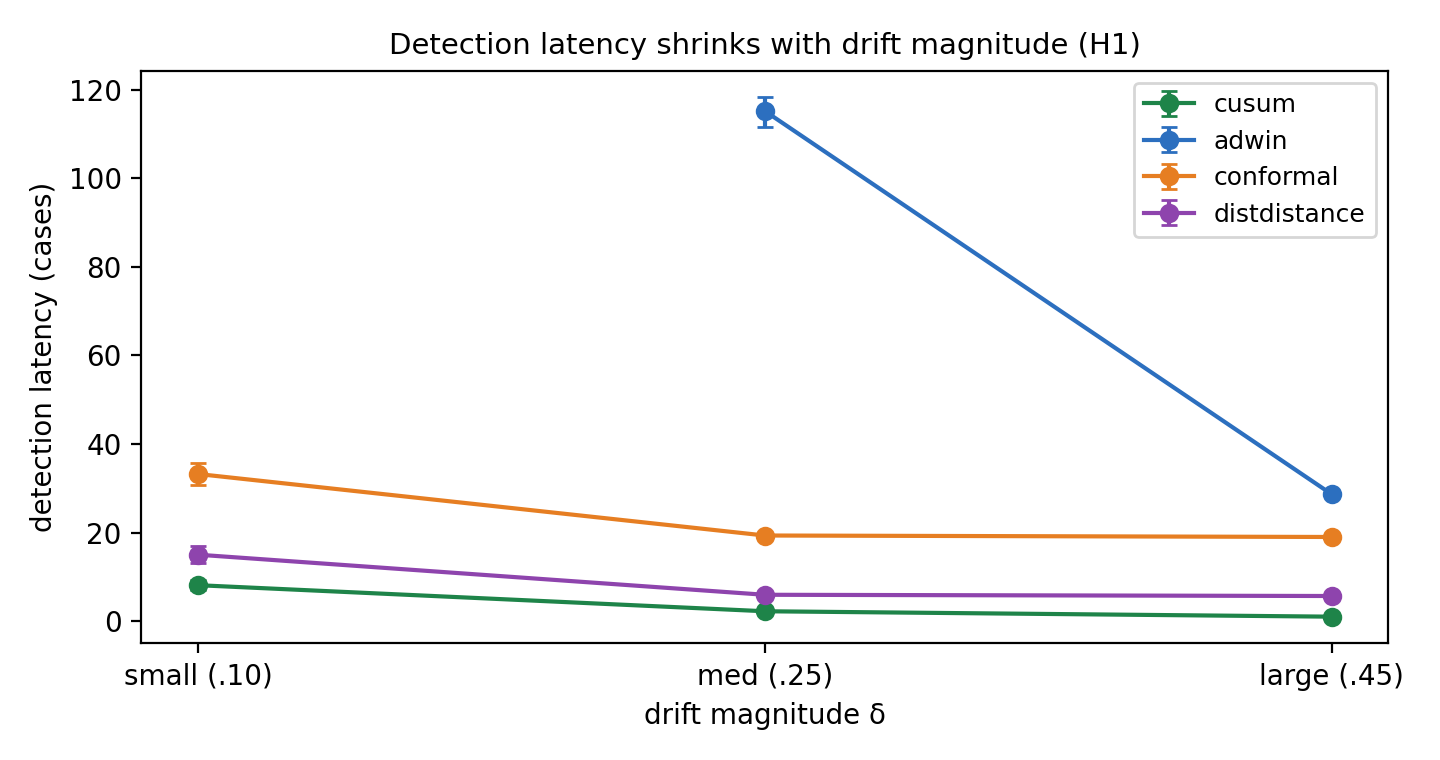
\includegraphics[width=0.95\linewidth]{figs/e1_latency_vs_magnitude.png}
\caption{\textbf{The paper in one figure.} Detection latency (cases from the true onset to
the first alarm; bootstrap 95\% CI) versus injected drift magnitude $\delta$, for four
sequential detectors on HAARF-Drift. CUSUM and the distributional-distance monitor catch
even small drift in a handful of cases; the conformal martingale is steady; ADWIN is
\emph{robust but conservative} --- it misses the smallest drift entirely (no point at
$\delta{=}0.10$) and pays a long latency at medium $\delta$. No single detector dominates,
which is the design argument: a deployment monitor should run \emph{several} complementary
detectors rather than bet on one. Every detector here works from a cheap proxy signal and
needs no labels.}
\label{fig:hero}
\end{figure}

A review of related work reveals three families (Table~\ref{tab:related}): periodic
batch re-evaluation, streaming concept-drift detectors from the ML-systems literature,
and emerging AI-autonomy/post-market frameworks. The recurring gap is that none is wired
\emph{into a clinical agent gateway as an always-on, adversary-aware, label-robust layer}.

\paragraph{Contributions.}
\begin{enumerate}
  \item \textbf{The central result.} On HAARF-Drift, no single drift detector dominates,
  and outcome-based monitoring \emph{degrades under delayed/partial labels} (detection
  \EtwoFullRate{}$\to$\EtwoSparseRate{}, latency \EtwoFullLat{}$\to$\EtwoMaxLat{} cases),
  while a \emph{label-free} behavioral monitor holds at \BehRecall{} recall, \BehFPRop{}
  FPR --- so deployment-time safety requires several complementary signals, including an
  unsupervised one.
  \item \textbf{The system.} \texttt{qfire monitor}: four sequential, memory-bounded drift
  detectors (CUSUM, ADWIN, conformal-martingale, distributional-distance), an autonomy
  meter against an authorized envelope, an unsupervised per-agent behavioral baseline, a
  graduated alert ladder, and a real-world-evidence exporter --- all off the hot path.
  \item \textbf{The benchmark.} \textbf{HAARF-Drift}: \NumPrompts{} deterministic,
  fully synthetic temporal streams (\StreamLen{} cases each) with labeled, injected drift,
  autonomy-creep, and behavioral-anomaly episodes of known onset and magnitude, released
  with a one-command regenerator.
  \item \textbf{Deployment evidence.} The whole monitor runs at sub-\textmu s to
  \OvDist~\textmu s per event with bounded memory (\S\ref{sec:overhead}); it is an
  off-hot-path read-side over an existing signed log, so it imposes no per-call cost.
\end{enumerate}

\paragraph{Positioning.} The closest prior line is the streaming concept-drift
literature~\cite{page1954cusum,bifet2007adwin,gama2014survey,volkhonskiy2017conformal}.
We do not invent a new detector; we ask which of these classical detectors actually serve
a \emph{clinical agent gateway} under late labels and adversarial drift, and we wire the
answer in as an always-on layer that feeds the program's oversight~\cite{policy2026} and
lifecycle machinery.

% ============================================================================
\section{Problem Setting}\label{sec:problem}
We monitor a stream of agent decisions. The deployment failure modes are:

\begin{itemize}
  \item \textbf{D1 Performance drift.} Outcome quality declines over time --- covariate
  shift, label shift, or a silent upstream-model update.
  \item \textbf{D2 Autonomy creep.} The agent acts autonomously more often, or on
  higher-risk actions, than its authorized envelope permits.
  \item \textbf{D3 Behavioral anomaly.} A sudden shift in tool-use or decision patterns
  (compromise, misconfiguration) with no labeled outcome to confirm it.
  \item \textbf{D4 Silent failure.} Degradation is invisible because labeled outcomes
  arrive late or not at all. D4 is a \emph{modifier} on D1--D3, not a separate stream ---
  it is the regime that defeats batch evaluation.
\end{itemize}

\paragraph{Signals.} The monitor reads a \texttt{MonitorEvent} per decision. In deployment
this is \emph{joined} from a signed audit record~\cite{tamperaudit2026} --- which already
carries a timestamp, the terminal verdict, the maximum detector score, and per-node
latency --- plus three fields fed back out of band: a possibly-lagged clinical outcome
(D1/D4), the autonomy level/risk tier of the action taken (D2), and the agent identity and
tool invoked (D3). The benchmark emits the joined event directly so the detectors are
exercised exactly as on the deployed read-side path.

\begin{table}[htb]\centering\small
\begin{tabular}{L{3.2cm}L{4.3cm}L{4.3cm}}
\toprule
Approach & What it does & Gap this paper targets \\
\midrule
Periodic batch re-evaluation~\cite{finlayson2021clinician} & re-score against a labeled set on a schedule & late labels; misses pre-outcome drift; not continuous \\
Streaming drift detectors~\cite{page1954cusum,bifet2007adwin,volkhonskiy2017conformal} & sequential change detection on a data stream & not wired to an agent gateway; no autonomy/behavioral/adversarial framing \\
AI lifecycle / SaMD frameworks~\cite{fda2021samd,schwoebel2026haarf} & require post-market monitoring & specify \emph{that}, not an always-on \emph{mechanism} \\
\textbf{This work} & off-hot-path, multi-signal, label-robust monitor in the gateway & --- \\
\bottomrule
\end{tabular}
\caption{Positioning against representative approaches to keeping a deployed model safe.}
\label{tab:related}
\end{table}

% ============================================================================
\section{System Design}\label{sec:design}
\subsection{Overview and components}
\texttt{qfire monitor} (Rust, \MonitorTests{} unit tests) is a read-side consumer of the
signed decision stream. It comprises: \textbf{four drift detectors} over a scalar proxy
signal, an \textbf{autonomy meter}, an \textbf{unsupervised behavioral baseline}, a
\textbf{graduated alert ladder}, and a \textbf{real-world-evidence (RWE) exporter}. Every
drift detector implements one sequential interface --- \texttt{observe(case, x)} returning
an optional \texttt{DriftSignal} --- and is memory-bounded (CUSUM $O(1)$; ADWIN
$O(\log n)$ buckets; conformal/distance $O(\text{window})$). This is the deployability
claim: the monitor is a constant- or log-space pass over a stream.

\paragraph{Drift detectors.} (1) \textbf{CUSUM}~\cite{page1954cusum} accumulates two-sided
cumulative sums of the proxy against an in-control mean with slack $k$ and threshold $h$.
(2) \textbf{ADWIN}~\cite{bifet2007adwin} maintains an exponential histogram and shrinks an
adaptive window whenever a Hoeffding-bounded mean difference is significant. (3) The
\textbf{conformal martingale}~\cite{volkhonskiy2017conformal,vovk2005algorithmic} bets on
conformal $p$-values; by Ville's inequality the betting martingale bounds the false-alarm
rate by $\alpha$ under exchangeability~\cite{shafer2019game}. (4) \textbf{Distributional
distance} compares a fixed reference histogram to a sliding window via the population
stability index or a Kolmogorov--Smirnov statistic. They embody four different assumptions
about \emph{what changed}, which is why they are complementary (\S\ref{sec:results}).

\paragraph{Autonomy meter.} An \texttt{AutonomyEnvelope} (maximum autonomous risk tier,
maximum autonomous fraction over a window) models the surface the forthcoming regulatory
passport will supply. The meter flags an action that is autonomous above the authorized
tier immediately, and flags sustained autonomous-fraction creep over the window.

\paragraph{Behavioral baseline.} For each agent, a categorical tool-use profile is learned
over a warmup window; a sliding window is then scored against it by population-stability
divergence (a previously-unseen tool is a strong signal). This path uses \emph{no labels}
and is the answer to D4.

\paragraph{Graduated alert ladder.} Detector severity maps to \texttt{log}~$\to$~%
\texttt{notify}~$\to$~\texttt{throttle}~$\to$~\texttt{halt}. The ladder tallies per-level
volume so that only the clinician-facing levels (notify/throttle/halt) count against an
alert-fatigue budget --- the seam to the program's oversight router.

\begin{figure}[htb]\centering
\begin{tcolorbox}[policycard, cardcol=cardteal, title=The monitor as an off-hot-path
  consumer, width=0.86\linewidth]
\begin{lstlisting}[style=housespecyamlbare]
signed decision stream (quledger)  -->  MonitorEvent (+ outcome, autonomy, tool)
  drift:    cusum | adwin | conformal | distdistance   (proxy signal, no labels)
  autonomy: meter vs authorized envelope               (risk tier + fraction)
  behavior: per-agent baseline                         (unsupervised, D4)
  ladder:   log -> notify -> throttle -> halt          (clinician budget)
  rwe:      export evidence -> passport / equity reporter
\end{lstlisting}
\end{tcolorbox}
\caption{The monitor reads the signed decision stream off the hot path and runs each
signal independently, so it adds no per-call latency and degrades gracefully if a feed is
late.}
\label{fig:arch}
\end{figure}

\subsection{Implementation}
The module is \texttt{src/monitor/} in the gateway crate; a \texttt{qfire monitor
-{}-stream} subcommand replays a decision stream through the detectors and prints the alert
ladder plus an RWE summary. All experiments run offline over HAARF-Drift via a
\texttt{driftbench} binary. Everything is deterministic given the seed.

% ============================================================================
\section{HAARF-Drift}\label{sec:benchmark}
Existing drift benchmarks~\cite{koh2021wilds} target image/tabular distribution shift, not
\emph{temporal agent-decision streams with autonomy and behavioral structure}, and contain
no labeled adversarial creep. We therefore build \textbf{HAARF-Drift}: \NumPrompts{}
deterministic, fully synthetic streams (\StreamLen{} cases each; seed \Seed{}), released
with a one-command regenerator.

\begin{itemize}
  \item \textbf{Drift} (\DriftOnset{} onset + \DriftClean{} clean): an outcome-failure
  proxy in $[0,1]$, stationary then a step of known magnitude
  $\delta\in\{0.10,0.25,0.45\}$ at a labeled onset $t_0$, across three families ---
  covariate (variance inflation), label (mean step), and model-update (step) shift.
  \item \textbf{Autonomy} (\AutoCreep{} creep + \AutoClean{} clean): per-case autonomous
  flag and risk tier; creep raises the autonomous fraction and tier past the envelope at
  $t_0$.
  \item \textbf{Behavior} (\BehAnom{} anomaly + \BehClean{} clean): per-case tool; an
  anomaly injects an abrupt tool-distribution shift (a previously-unseen tool) at $t_0$.
\end{itemize}

A sidecar records, per stream, the onset index, magnitude, and type. All data are
synthetic; no protected health information is used.

% ============================================================================
\section{Experiments and Results}\label{sec:results}
We measure detection latency (cases from $t_0$ to the first alarm at or after onset; an
alarm before $t_0$ or on a clean stream is a false alarm). Rates carry Wilson 95\%
CIs~\cite{wilson1927}; latencies carry bootstrap 95\% CIs; ROC/AUC sweeps each detector's
threshold.

\subsection{E1 --- drift detection and the no-dominator result}
At their operating points all detectors except ADWIN detect every onset
(\CusumDet{}, \ConfDet{}, \DistDet{}); ADWIN detects \AdwinDet{} because its conservative
Hoeffding bound misses the smallest magnitude. Detection latency shrinks with magnitude
(Figure~\ref{fig:hero}): CUSUM falls from \CusumLatSmall{} cases at $\delta{=}0.10$ to
\CusumLatLarge{} at $\delta{=}0.45$; the distance monitor from \DistLatSmall{} to
\DistLatLarge{}; the conformal martingale is steady around \ConfLatLarge{}; ADWIN pays
\AdwinLatMed{} cases at medium $\delta$. The ROC (Figure~\ref{fig:roc}) confirms the
picture: AUC \CusumAUC{} (CUSUM), \ConfAUC{} (conformal), \DistAUC{} (distance), and
\AdwinAUC{} (ADWIN). \emph{No single detector dominates}: CUSUM is best for mean shifts,
the distance monitor is fast and catches variance-only (covariate) drift that a mean
detector cannot, the conformal martingale gives a distribution-free false-alarm guarantee,
and ADWIN is the most conservative. This is why the monitor runs all four.

\begin{figure}[htb]\centering
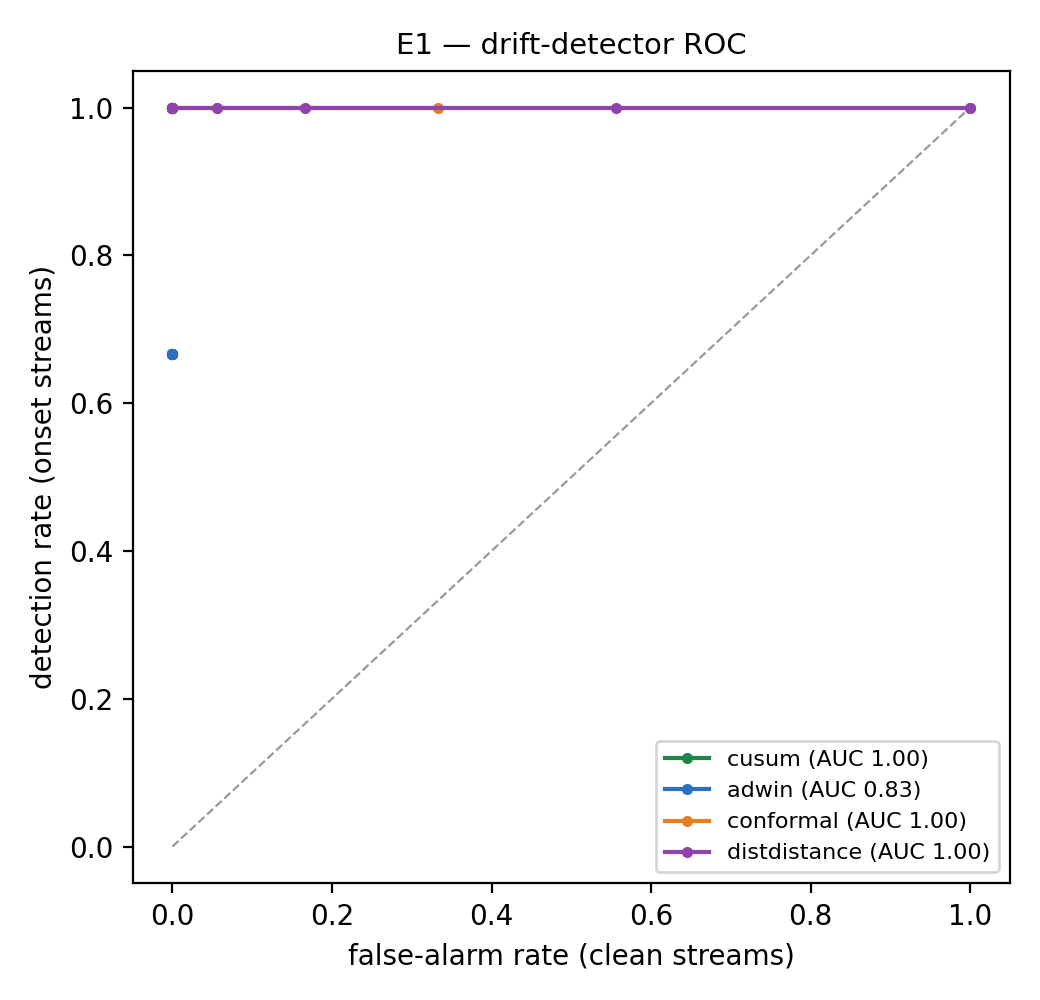
\includegraphics[width=0.62\linewidth]{figs/e1_roc.png}
\caption{\textbf{E1 ROC.} Detection rate over onset streams versus false-alarm rate over
clean streams, sweeping each detector's threshold. CUSUM, conformal, and distance reach
the top-left corner (AUC \CusumAUC{}); ADWIN tops out at AUC \AdwinAUC{} because it cannot
catch the smallest drift at any threshold without alarming on clean streams.}
\label{fig:roc}
\end{figure}

\subsection{E2 --- delayed and partial labels (D4)}
We feed the \emph{outcome}-based signal to CUSUM and vary label delay and label fraction
(Figure~\ref{fig:e2}). With full, immediate labels, outcome-CUSUM detects \EtwoFullRate{}
of onsets at latency \EtwoFullLat{} cases. Delay adds directly to latency
(\EtwoDelayLat{} cases at a 150-case delay) and sparsity both raises latency and lowers
recall (\EtwoSparseRate{} at a 20\% label fraction; up to \EtwoMaxLat{} cases combined),
all at a false-alarm rate $\le\EtwoMaxFAR{}$. Crucially, recall \emph{caps at
\EtwoFullRate{}} even with perfect labels, because covariate-family drift inflates variance
without yet moving the mean outcome --- a proxy-validity failure that outcome monitoring
cannot escape. This is the quantitative case for not relying on labeled outcomes alone.

\begin{figure}[htb]\centering
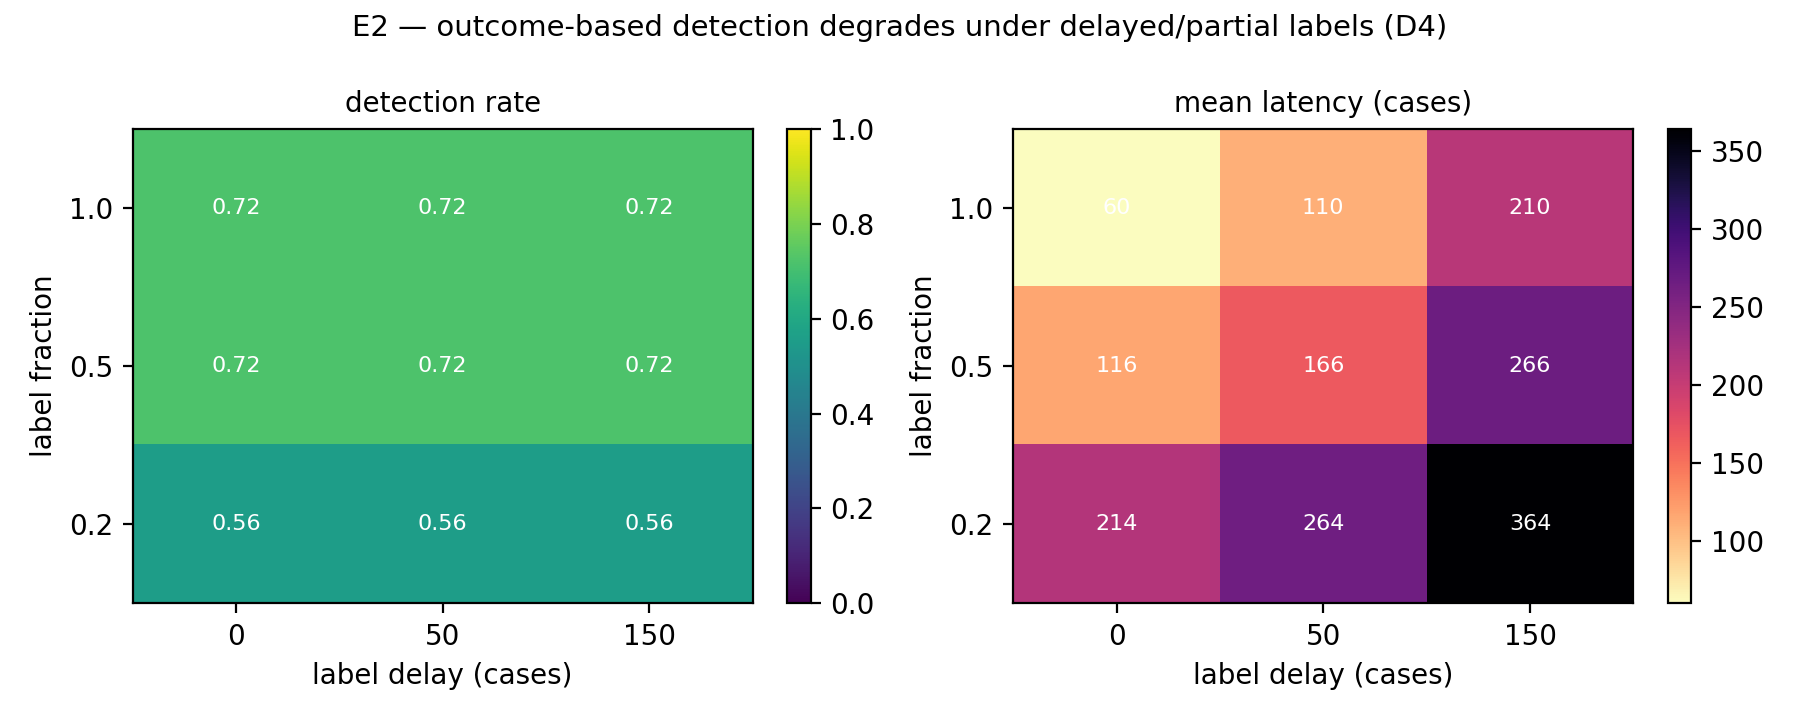
\includegraphics[width=0.95\linewidth]{figs/e2_delayed_labels.png}
\caption{\textbf{E2 --- outcome-based detection degrades under D4.} Detection rate (left)
and mean latency (right) as label delay (columns) and label fraction (rows) vary. Latency
grows with both; recall falls with sparsity and is capped by covariate drift that outcomes
do not reflect --- motivating the label-free behavioral path (E4).}
\label{fig:e2}
\end{figure}

\subsection{E3 --- autonomy creep}
Against authorized envelopes spanning maximum autonomous fractions
\AutoEnvLo{}--\AutoEnvHi{}, the autonomy meter catches creep at \AutoRecall{} recall and
\AutoFAR{} false-alarm rate, with a latency of \AutoLat{} cases past onset
(Figure~\ref{fig:e3}) --- because a single autonomous action above the authorized tier is
flagged immediately. This is the clean case: autonomy is observable directly, without
labels and without ambiguity, so it should be monitored directly rather than inferred from
outcomes.

\begin{figure}[htb]\centering
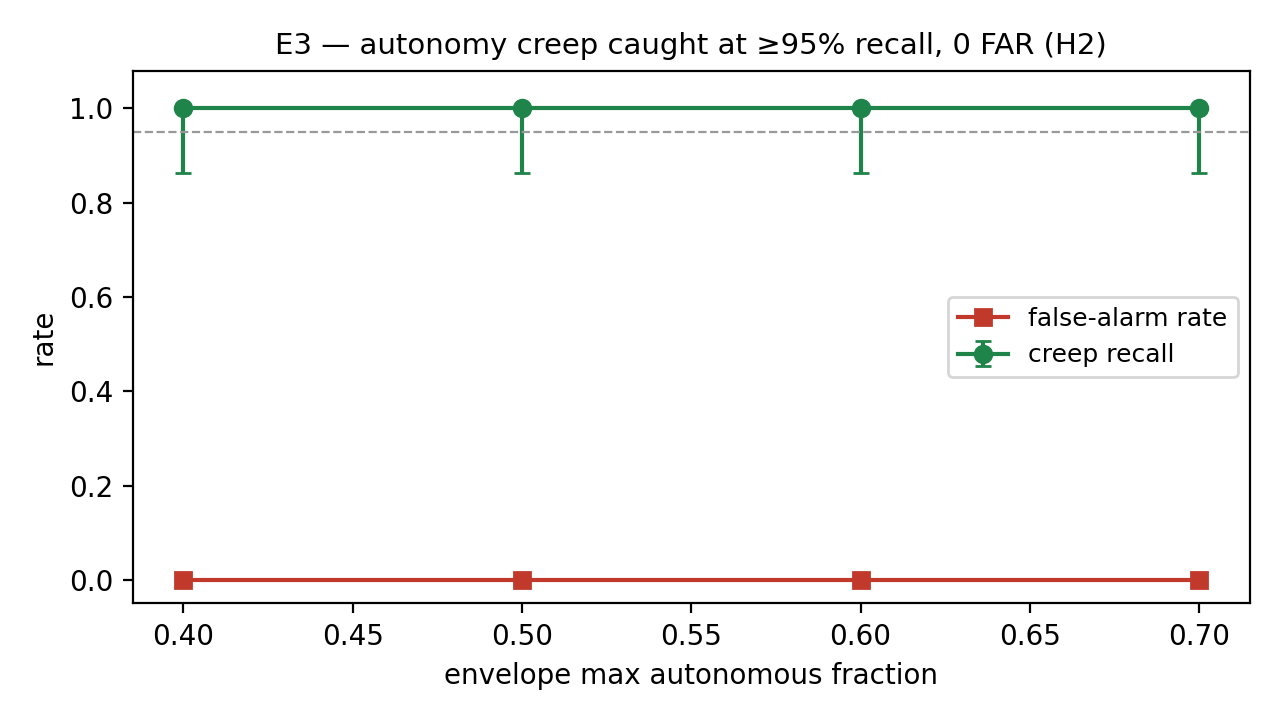
\includegraphics[width=0.6\linewidth]{figs/e3_autonomy.png}
\caption{\textbf{E3 --- autonomy creep.} Creep recall (Wilson 95\% CI) and false-alarm
rate versus envelope tightness. Recall is \AutoRecall{} at \AutoFAR{} false alarms across
the swept envelopes (dashed line: 95\% target).}
\label{fig:e3}
\end{figure}

\subsection{E4 --- unsupervised behavioral anomaly}
The behavioral baseline uses no labels. Sweeping its threshold (Figure~\ref{fig:e4}), it
reaches \BehRecall{} recall throughout; at the operating threshold \BehThreshOp{} the
false-positive rate is \BehFPRop{} (zero for any threshold $\ge 0.35$) at a latency of
\BehLatOp{} cases. Only an over-sensitive threshold (0.2) inflates the FPR (to
$\approx\BehFPRsens{}$). Where outcome monitoring stalls under D4 (E2), this label-free
signal holds --- the two paths are complementary, which is the structural argument of the
paper.

\begin{figure}[htb]\centering
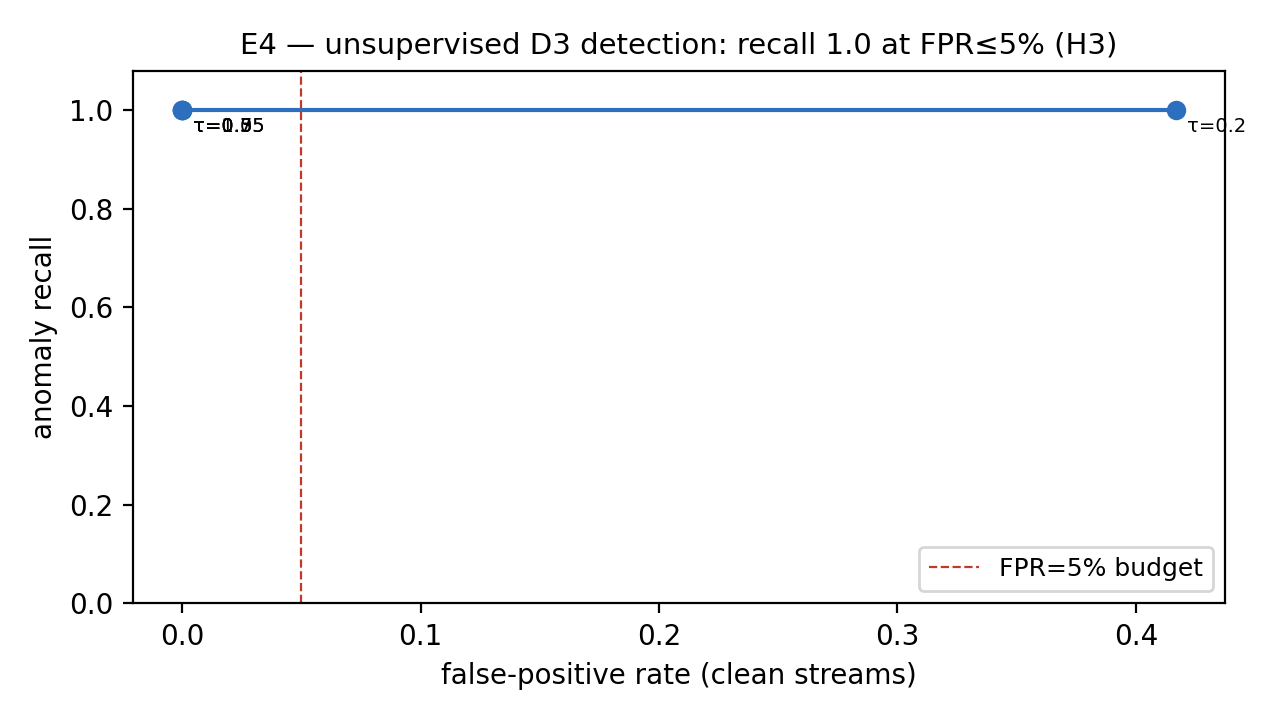
\includegraphics[width=0.6\linewidth]{figs/e4_behavior.png}
\caption{\textbf{E4 --- unsupervised behavioral detection.} Anomaly recall versus
false-positive rate as the threshold varies; the operating point sits at recall
\BehRecall{}, FPR \BehFPRop{}, well inside the 5\% budget (dashed line). No labels are
used.}
\label{fig:e4}
\end{figure}

\subsection{E5 --- monitoring overhead}\label{sec:overhead}
Over \OvEvents{} events, per-event cost is \OvCusum~\textmu s (CUSUM), \OvConf~\textmu s
(conformal), \OvAdwin~\textmu s (ADWIN), and \OvDist~\textmu s (distance)
(Figure~\ref{fig:e5}); ADWIN's resident state stays bounded at \AdwinBuckets{} buckets.
Because the monitor consumes the signed log off the hot path, this cost is never on the
request critical path: the deployment imposes \emph{no} per-call latency.

\begin{figure}[htb]\centering
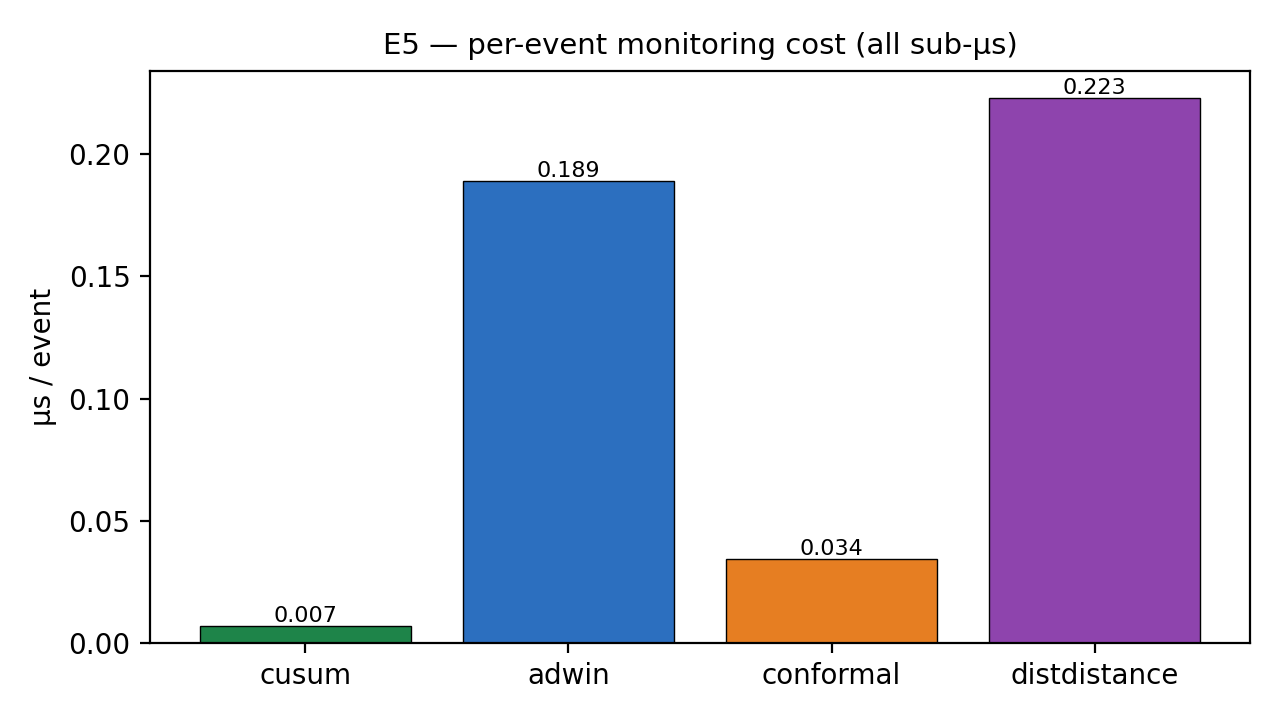
\includegraphics[width=0.6\linewidth]{figs/e5_overhead.png}
\caption{\textbf{E5 --- overhead.} Per-event monitoring cost for each detector; all are
sub-microsecond to a fifth of a microsecond, with bounded memory.}
\label{fig:e5}
\end{figure}

% ============================================================================
\section{Discussion and Limitations}\label{sec:limits}
\paragraph{Interpretation.} The results say something simple and a little
uncomfortable: there is no one detector to deploy. Mean-shift, variance-shift,
exchangeability, and distributional detectors each catch what the others miss, and the
signal that survives the silent-failure regime (D4) is the \emph{unsupervised} behavioral
one --- precisely because an adversary degrading an agent will avoid moving the labeled
outcome for as long as possible. A deployment monitor is therefore a small \emph{ensemble}
of cheap detectors plus a label-free baseline, not a single statistic.

\paragraph{Relationship to HAARF.} The layer realizes continuous performance monitoring
(C1.4) and real-world evidence (C1.5) via the drift detectors and RWE exporter, autonomy
performance monitoring (C6.6) via the autonomy meter, and behavioral anomaly detection
(C5.5) via the unsupervised baseline~\cite{schwoebel2026haarf}. The graduated ladder is the seam to
the oversight router, and the RWE exporter is the seam to the regulatory passport and
equity reporter.

\paragraph{Limitations.} HAARF-Drift is synthetic: it lets us control onset and magnitude
exactly and reason about detection latency, but real clinical streams will have richer,
confounded structure, and the proxy-signal-validity threat (E2's ceiling) is more severe
in practice. The authorized envelope and the alert router are modeled locally; wiring them
to the real passport and oversight layers is the subject of the companion papers. We
report detection latency on injected step/episode drift; gradual ramps and recurring
seasonal drift are future work. Finally, the adversary here is a behavioral one --- an
attacker who can also forge the monitored feed is out of scope and is the province of the
signed-audit layer~\cite{tamperaudit2026}.

% ============================================================================
\section{Conclusion}
A clinical agent that passes review can still fail in the field, and the failures that
matter most are the ones that hide from labeled outcomes. \texttt{qfire monitor} watches
the deployment rather than the call: an off-hot-path ensemble of sequential,
memory-bounded detectors for drift, autonomy creep, and behavioral anomaly, plus an
unsupervised path for the silent-failure regime, at sub-microsecond per-event cost. The
next steps consume its output: the regulatory passport ingests its real-world evidence to
gate change, and the oversight router consumes its graduated alerts to route only
genuinely ambiguous cases to clinicians.

% ============================================================================
\section*{Declaration of generative AI use}
During the preparation of this work the authors used \emph{Anthropic Claude (Claude Code)}
for drafting boilerplate, generating and debugging the Rust monitor module, the synthetic
data generator, and the figure-plotting code, and for copy-editing. After using this tool,
the authors reviewed and edited the content and take full responsibility for the
publication. No generative-AI system was used to generate or fabricate data, interpret
results, or produce clinical conclusions, and no AI tool is listed as an author, as such
tools do not satisfy authorship criteria.

\section*{Data and code availability}
All code, the HAARF-Drift generator, the \texttt{driftbench} harness, and the analysis
scripts are available at
\href{https://github.com/quome-cloud/qudrift}{\nolinkurl{github.com/quome-cloud/qudrift}}.
All patient data are synthetic; no real protected health information was used.

\section*{Author contributions}
J.S. and the QUOKKAGUARD contributors conceived the study, designed and implemented the monitor layer and
benchmark, ran the experiments, and wrote the manuscript; all authors reviewed and approved
it.

\section*{Competing interests}
The authors declare no competing interests.

\section*{Funding}
This work received no specific external funding.

% ============================================================================
\appendix
\section{Reproducibility}\label{app:reproduce}
From a checkout of the repository:
\begin{lstlisting}[style=housespecyamlbare]
python3 scripts/011-drift-monitoring/gen_drift.py        # HAARF-Drift (seed 42)
cargo run --release --bin driftbench -- --exp all        # E1-E5 -> results/011-*
python3 scripts/011-drift-monitoring/summarize.py        # CIs, ROC/AUC, figures
cd papers/011-drift-monitoring && make paper             # this PDF
\end{lstlisting}
Every figure and number regenerates from the seeded run; detection metrics are
deterministic, and per-event timings (E5) are the only run-dependent quantities.

\clearpage
\bibliographystyle{plain}
\bibliography{refs}
\end{document}
